\documentclass{acm_proc_article-sp}

\usepackage{amsmath}
\usepackage{verbatim}
\usepackage{textcomp}
\usepackage{graphicx}
\usepackage{subcaption}
\usepackage{url}
\usepackage{multicol}
\usepackage{tikz}
\usetikzlibrary{positioning}
\usepackage{wasysym}
\setlength{\parindent}{1cm}
\usepackage{indentfirst}


\begin{document}

\title{Anonymous Reserve Auction Revenue Bounds \\
{\normalsize Code available at: \url{https://github.com/blasch/AnonymousReserve}}} 
\subtitle{}

\numberofauthors{2} 
\author{
% 1st. author
\alignauthor 
Robert Schneidman \\
	\affaddr{260476707}
% 2nd. author
\alignauthor Benjamin La Schiazza\\
	\affaddr{260531181}
% 3rd. author
}

\date{Nov30}

\maketitle
\begin{abstract}

\end{abstract}

\section{Introduction}
Auction theory is an incredibly relevant field to investigate as it has many modern applications. Society has been running auctions for centuries yet only now with advances in computing technology and mathematics have they been explored in an academic setting. A number of fundamental results have emerged from applying mathematical models to these settings. While some results are incredibly practical and have shaped business models, others remain inapplicable due to their inherent assumptions. 

One of these assumptions involves the nature of the distributions bidders choose they value for an object from. A very common practice is to assume all bidders pick values from the same distribution. In modern auctions settings found especially on the internet, bidders can come from a range of cultures and demographics and makes the applicability of theory stemming from these results not practical. Another fact in the basic auction revenue theory (eg. Myerson's Lemma[1]) is that to achieve optimal revenue, bidders must be assigned bidder specific reserves[2]. While this may be feasible when all bidders have identical distributions (meaning their reserves turn out to be the same), in realistic settings with multiple distributions, it is hard to justify to real bidders that certain participants have a lower or higher reserve to meet to be eligible in the auction. In the name of fairness, though to the determinant of obtaining optimal revenue, real auctions (eg. Ebay) employ a general reserve for all participants. Some general bounds have been noted regarding the approximation of optimal revenue with anonymous reserves but they are not tight\cite[p. 126]{hartline}. 

Due to the prevalence of Anonymous reserve auctions it is important to understand what kind of performance can be expected from their utilization. Our goal with this project was to explore and try and improve guarantees made on the optimal revenue approximations. More specifically, we aim to improve the upper bound proposed by Hartline (Lemma 4.17)\cite{hartline}. If a setting can be found under which the max revenue for anonymous reserve is significantly under 50\% then the possibility of formally improving the bound is there. The simplest setting we can do our investigation under is an auction with one item and two bidders.

\section{Theory}
Our ultimate goal is to make statements about the nature of the revenue one can expect when running a single-item Vickrey auction with an anonymous reserve. The bayesian optimal auction is used as a benchmark. It is appropriate however to lay some foundation before discussion the problem at hand.

\subsection{Dominant Strategy Incentive Compatible}
An auction is Dominant Strategy Incentive Compatible (DSIC) if bidding truthfully is the single strategy that will maximizes a bidder's utility. If an auction is DSIC, bidding truthfully will never result in a bidder having a negative utility function.

\subsection{Virtual Value}
Bidder i's \emph{virtual value} function is
\[ \phi_{i}(v) = v - \frac{1-F_{I}(v)}{f(_{I}v)}\] \\
Myerson showed in 1981 that in a single dimensional setting, given a distributions $F_i$ for each bidder, the expected revenue from a DSIC [5] mechanism is 
\[ E[\sum_{i} p_{i}(v)] = E[\sum_{i} x_{i}(v)\phi_{i}(v_{i})] \] \\
 In order to optimize revenue, a mechanism should allocate goods according to the virtual value function.

\subsection{Single-Item Vickrey Auction with Anonymous Reserve}
A single-item Vickrey auction with anonymous reserve is an auction where the winner is the bidder with the highest bid under the condition that he meets his reserve. He pays the maximum of his reserve price and the second highest bid. This auction is dominant strategy incentive compatible.

\subsection{Single-Item Bayesian Optimal Auction}
The single-item Bayesian optimal auction is an auction where the winner is the bidder with the highest virtual value under the condition that he meets his reserve.  The bidder specific reserve price is set at \[ r = \phi_{i}^{-1}(0)\] for each bidder i in order to maximize virtual welfare (that in turn maximizes expected revenue). The winning bidder pays the maximum price he would need to bid in order to no longer win the auction. This auction is dominant strategy incentive compatible. [7] It is the revenue maximizing auction under the condition that all bidder distributions are regular. 

\subsection{Regular Distributions}
The distributions we will explore are called Regular distributions and are defined as functions whose virtual value functions are non-decreasing. This restriction on distributions allows the Bayesian optimal auction to remain DSIC. It prevents bidders from increasing their chances of being allocated the item by lowering their bid.

Distributions in this class include the normal distribution, exponential distribution and uniform distribution. "Fat-tailed" distributions, defined as having a probability distribution
\[  f(x) \sim x^{-(1 + \alpha)} \: as \: x \rightarrow \infty ,\: \alpha > 0 \] \\ also belong to the class of regular distributions. A fat-tailed distribution with $\alpha = 1$ is known as the equal-revenue distribution. It lies on the boundary of regularity as it's virtual value function is constant. For the entirety of it?s domain, the virtual value function has a value of 0 and the expected posted price revenue is 1.

\subsection{Proof of Upper Bound on Anonymous Reserve Auction}
In Hartline's book draft [3], Lemma 4.18 proves an upper bound of 50\% on the anonymous reserve auction. Hartline designs a mechanism with a single equal-revenue bidder with an arbitrarily large reserve price and a second bidder who bids 1 with probability = 1. This mechanism has an optimal revenue of 2.  An anonymous reserve auction will have an expected revenue of 1 regardless of how the reserve price is set. 

\section{Methodology}
Our approach to explore this topic was two-fold. The first step was eliminating auctions that exceed the 50\% approximation when assigned a particular anonymous reserve. These auctions were removed from the sample space and an exhaustive search was performed over 2 and 3 bidder auctions within the remaining sample space.




By setting up an auction between various types of bidders, calculating the expected revenue under anonymous reserves and the optimal revenue, we can search for situations were the ratio of anonymous reserve revenue to optimal revenue is under 50\%.

\subsection{Bidder Distributions}
The initial pool of bidders had the following underlying regular distributions: uniform, exponential, gamma, normal, equal revenue distribution (ERD), fat-tailed distributions with alpha equal to two, three and four and finally a bidder that always bids 1. 

\subsection{Setting Bidder Specific Optimal Reserves}

Initially, the process of finding the  bidder specific reserve was done by an exhaustive search method. All values x where 0 < cdf(x) < 1 were tested in order to maximize the single item single bidder posted price revenue. The calculation was done this way because many distributions do not have a closed form solution for finding $\phi^{-1}(0)$. Eventually, the process of setting a bidder specific reserve was done using a library function which was able to solve for $\phi^{-1}(0)$. This change allowed us to reduce the error when calculating the optimal revenue since the search increments were not infinitesimally small.

\subsection{Setting Anonymous Reserves}
	The minimum anonymous reserve tested for a given auction was \[\min_{i}(F_i(v_0))\] where i is a bidder participating in the auction and $v_0$ is a value drawn from $F_i$ such that $F_i(v_0) = 0.001$.
	
	 The maximum anonymous reserve tested for a given auction was \[\max_{i}(F_i(v_0))\] where i is a bidder participating in the auction and $v_0$ is a value drawn from $F_i$ such that $F_i(v_0) = 0.999$.
	 
	The intervals between anonymous reserves that were tested was proportional to the range of candidate anonymous reserves. This was the most logical portion of the program to sacrifice precision. In most cases, a sub-optimal anonymous reserve exceeded the 50\% approximation (with error accounted for). In the case where the 50\% approximation was not met, the auction was tested a subsequent time with smaller intervals used to pinpoint the anonymous reserve. 
 
\subsection{Setting Number of Iterations of Each Auction}

After the reserve price was set, each auction was run proportional to the minimum probability of each bidder bidding above the reserve price . Each auction was run \[1000 *\frac{1}{\min_{i}(1- F_i(r))}\] where r is the anonymous reserve price in the anonymous reserve Vickrey auction and the bidder specific reserve price for bidder i in the Bayesian Optimal Auction.

No auction was run more then 10,000 times due to run time constraints. 

\subsection{Running the Experiment}

Auctions were created by exhaustively combining distributions that made up the sample space. Distributions were first grouped into groups of 2 to form 2-bidder auctions and then groups of 3 to form 3-bidder auctions. For each auction, after the bidder-specific reserves were found, the optimal auction was run to determine the benchmark. Then, the anonymous reserve Vickrey auction was run with varying reserve prices. When a reserve price was found where the 66.66\% benchmark was was met, no further reserve prices were tested. Any auction who's optimal anonymous reserve price revenue fell below 66.66\% of optimal revenue was stored for further testing.

\section{Results}

\subsection{Determining Error}

Several auctions were run under our experimental conditions and compared to the theoretical expected revenue to determine an appropriate error consideration. One of  these auctions was the auction from Hartline's upper bound proof. Anonymous reserve prices were tested between 1 and 5 and the following results were gathered.

	\begin{figure}[!htbp]
   		\centering
  		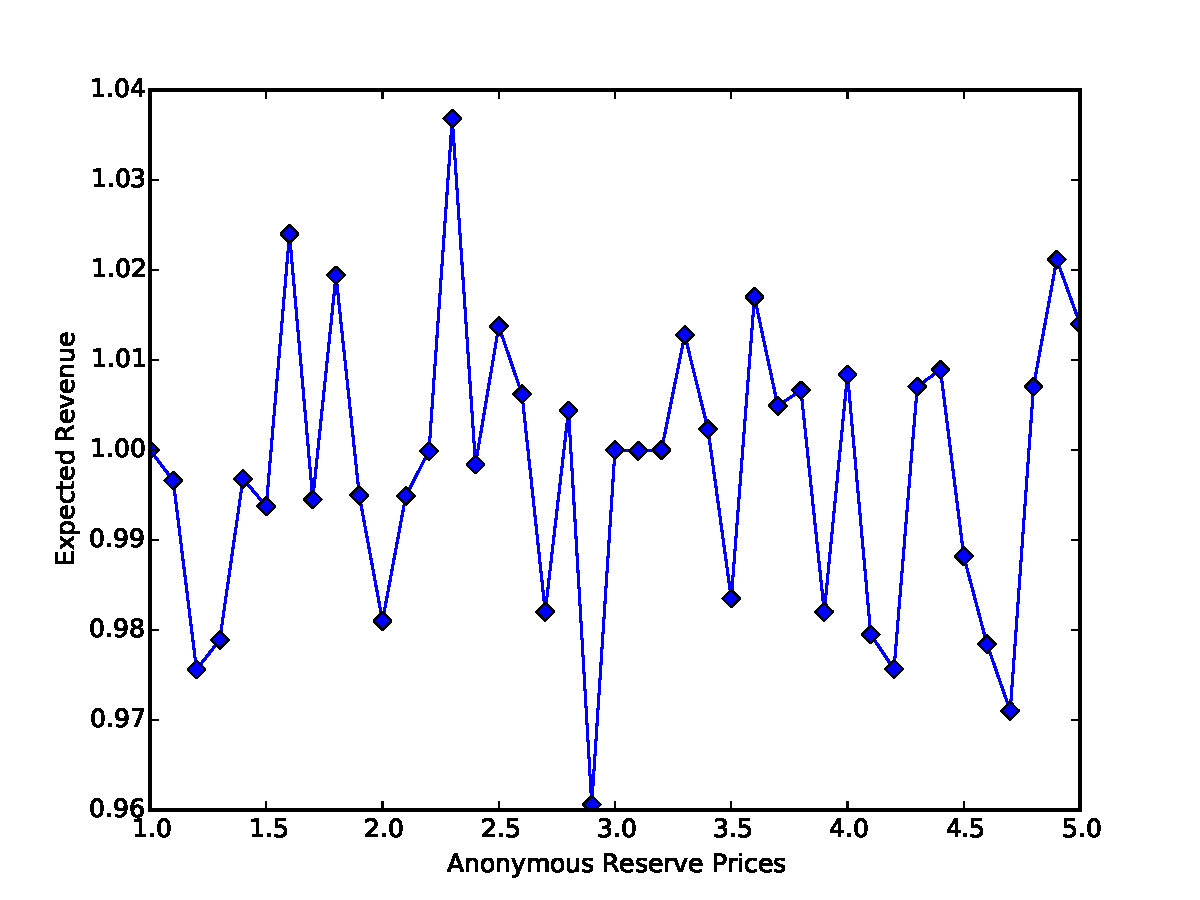
\includegraphics[width=\linewidth]{Hartline.pdf}
    		\caption{Expected Revenue from Hartline's Upper Bound Auction}
    		\label{Figure 1}
	\end{figure}
	
The expected revenue for all the anonymous reserve prices tested was 1. All 50 auctions fell within 4\% of the expected revenue. Throughout many simulations of the Bayesian Optimal Auction under our experimental conditions, the revenue outputted fell within 5\% of the theoretical expected revenue of 2.

Based on these experiments, a conservative error consideration of 10\% revenue was made for both the anonymous reserve auction and the optimal auction. This 10\% error for both auctions led to all auctions where the optimal anonymous reserve achieved less than 66\% of optimal revenue being considered as potentially improving the upper bound.

\subsection{Auctions related to Hartline's Upper Bound Proof}

Claim: Adding any 3rd bidder to Hartline's mechanism will not improve the 50\% approximation

Proof:

Case 1: Adding a second Equal Revenue Distribution to form a Mechanism M'

Proof: Adding a second Equal Revenue bidder with an arbitrarily large reserve price to the Bayesian Optimal Auction will contribute his posted price revenue of 1 to M' giving a total expected revenue of 3. The anonymous reserve Vickrey auction with an arbitrarily large reserve price will yield an expected revenue of 2. Both bidder's have a posted price revenue of 1 and the probability that both bidder's meet the anonymous reserve is 0. Therefore the anonymous Vickrey auction on M' has a lower bound of 2/3 of optimal revenue.

Case 2: Adding a bidder i with $\phi_i^{-1}(0) \geq 1$ to form a Mechanism M'

Proof: The third bidder will have an optimal reserve $r \geq 1$.  Setting the anonymous reserve in the Vickrey auction to be r will yield at least the posted price revenue of selling to the third bidder + 1. When the third bidder meets the reserve price r, M' will generate at least r and when he doesn't meet r, the expected revenue will be 1 



\subsection{Did we do better?}

Unfortunately this was the closest any of our simulated auctions got to the upper bound proposed. All other scenarios had ratios well closer to 1 of the optimal revenue. In fact all of the other pairings with an ERD produced (within error) a ratio around 1. One to highlight is an auction between two ERD. As they have identical distributions, the ratio was ~1 with Figure \ref{fig:erd2} showing data collected for anonymous reserve auction. The optimal expected revenue is theoretically 2 and the anonymous auction achieves approximately the same result.



\section{Discussion}

The results were clearly not very groundbreaking. The theoretical proof was re-implemented successfully and a large number of similar auctions involving a range of regular distributions were run. All the other results had approximations of the optimal revenue hovering around 100\%.

\section{Conclusion}

\begin{thebibliography}{9}

	\bibitem{hartline}
		"4 Bayesian Approximation." Mechanism Design and Approximation. N.p.: n.p., n.d. N. pag. Jason Hartline. N/A. Web. 6 Dec. 2014. <http://jasonhartline.com/MDnA/MDnA-ch1to6.pdf>.

\end{thebibliography}

\end{document}
